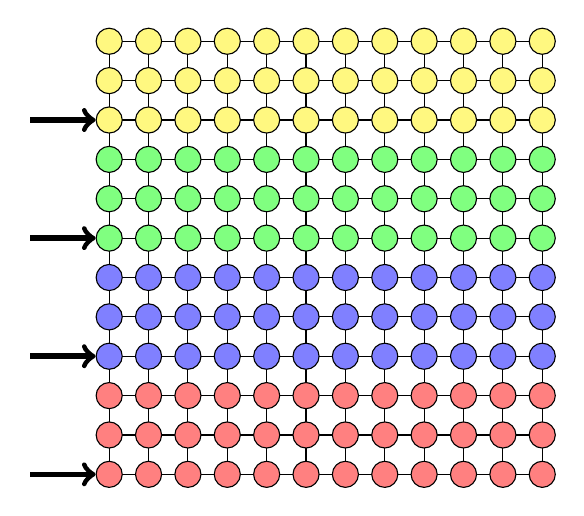
\begin{tikzpicture}[]
    \draw (0, 0) grid[step=0.5] (5.5,5.5);
    \foreach \x in {0,...,11} {
        \foreach \y in {0,...,2}  {
           \node [circle, draw, fill=red!50] (\x\y) at (0.5*\x,0.5*\y) {};
        }
        \foreach \y in {3,...,5} {
           \node [circle, draw, fill=blue!50] (\x\y) at (0.5*\x,0.5*\y) {};
        }
        \foreach \y in {6,...,8} {
           \node [circle, draw, fill=green!50] (\x\y) at (0.5*\x,0.5*\y) {};
        }
        \foreach \y in {9,...,11} {
           \node [circle, draw, fill=yellow!50] (\x\y) at (0.5*\x,0.5*\y) {};
        }
    }
    \draw[->,line width=2] (-1, 0) -- (00);
    \draw[->,line width=2] (-1, 1.5) -- (03);
    \draw[->,line width=2] (-1, 3) -- (06);
    \draw[->,line width=2] (-1, 4.5) -- (09);
\end{tikzpicture}